\chapter{Précautions}\label{ch:precautions}

Ce chapitre regroupe les règles de sécurité obligatoires qui accompagnent chaque bloc d'instruments \ReplicaGenOne{} et \ReplicaNextLong{}.
Ignorer l'un de ces points est le moyen le plus rapide d'endommager l'électronique ou d'obtenir des mesures peu fiables.

\begin{enumerate}
    \item \textbf{Débranchez la batterie du véhicule avant de commencer l'installation.} Travailler sur un faisceau alimenté peut sembler plus rapide, mais plusieurs tableaux de bord ont déjà été détruits par des courts-circuits provoqués par un faisceau sous tension.
    \item \textbf{N'alimentez jamais les entrées capteurs avec une source de tension externe.} Les voies de température du liquide de refroidissement, de température d'huile, de température extérieure et de niveau de carburant sont conçues pour des capteurs passifs uniquement. Même un test « inoffensif » au travers d'une résistance brûle l'électronique de mesure.
    \item \textbf{Souvenez-vous que les panneaux des générations~1 et~1.5 ne possèdent aucun fusible interne.} Le premier élément de protection est le fusible de 15~A du boîtier Volkswagen. Il réagit bien trop tard pour sauver le bloc compteur en cas d'erreur de câblage.
    \item \textbf{Protégez l'appareil de la lumière directe du soleil.} Une exposition prolongée décolore les segments LCD et réduit définitivement le contraste.
    \item \textbf{N'essayez pas de suralimenter le rétroéclairage LED.} Les générations~1, 1.5 et~2 utilisent un éclairage à courant constant. Si l'image de jour est trop sombre, ajoutez de l'ombrage autour de la casquette plutôt qu'augmenter le courant d'entraînement.
    \item \textbf{Méfiez-vous des résonances des compteurs de vitesse à câble.} Les entraînements mécaniques oscillent souvent entre 40 et 60~km/h. Installez le capteur électronique fourni---livré avec tous les kits Gen~1.5 et Gen~2 actuels---dès que possible.
    \item \textbf{Prévoyez des commandes MFA externes pour les tableaux de bord de génération~2.} Le capteur tactile à logo VW a été supprimé ; le changement de mode MFA doit donc venir de la commande de colonne de direction ou d'un autre interrupteur externe.
    \item \textbf{Tenez compte du courant de veille.} Un bloc de génération~2 consomme environ 11 à 13~mA sur la batterie du véhicule même lorsque le contact est coupé. Cette consommation au repos ne peut pas être réduite.
    \item \textbf{La consommation instantanée de carburant n'est pas installée en usine.} La fonctionnalité peut être rétrofitée sur les unités Gen~1 et Gen~1.5 en suivant les instructions ci-dessous, mais elle n'a pas été validée pour le matériel Gen~2.
        \displayurl{https://www.youtube.com/watch?v=qWqvYc9388U}
\end{enumerate}

\begin{figure}[htbp]
    \centering
    \begin{subfigure}{0.46\textwidth}
        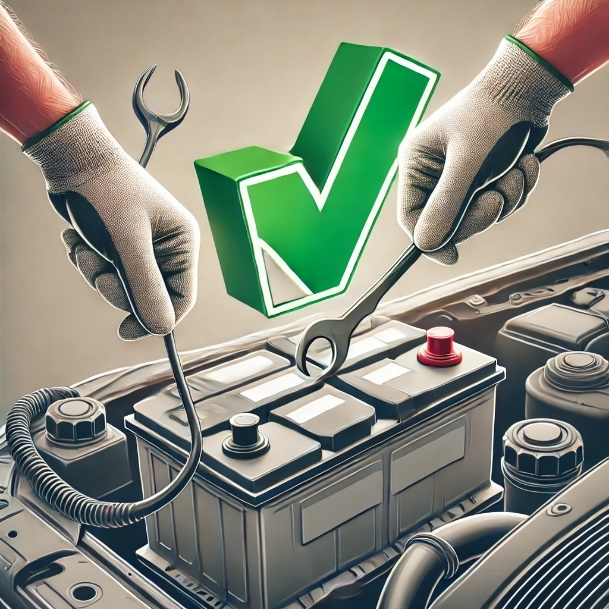
\includegraphics[width=\linewidth]{digifiz_manual/image001.jpg}
        \caption{Étiquette insistant sur la déconnexion de la batterie pendant l'installation.}
    \end{subfigure}\hfill
    \begin{subfigure}{0.46\textwidth}
        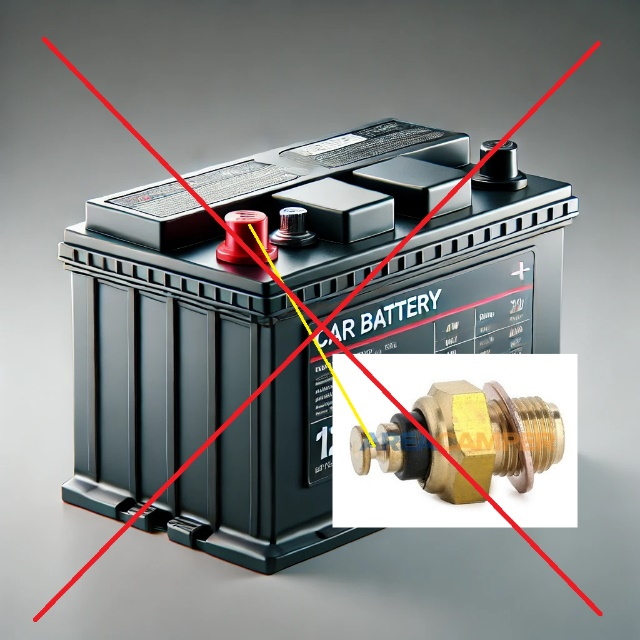
\includegraphics[width=\linewidth]{digifiz_manual/image002.jpg}
        \caption{Avertissement fourni avec le faisceau de capteurs contre toute tension externe.}
    \end{subfigure}
    \caption{Plaques de sécurité livrées avec le kit de câblage.}
\end{figure}
